\chapter{Introducción}

\section{Motivación}

\subsection{Evolución en los dispositivos de enrutamiento}

En un principio los enrutadores contaban con un bus central compartido, un CPU, memoria y los puertos de entrada y salida. Cada paquete entrante era transferido al CPU por medio del bus compartido. La decisión de forwarding se llevaba a cabo allí y luego el paquete atravesaba nuevamente dicho bus hacia el puerto de salida. La performance de estos dispositivos estaba limitada principalmente por 2 factores: la capacidad de procesamiento de la CPU central (debido a que la búsqueda en la tabla de ruteo es una tarea que consume una alta cantidad de tiempo) y el hecho de que cada paquete tenía que atravesar 2 veces el bus compartido.

Para hacer frente al primer factor algunos fabricantes de enrutadores introdujeron paralelismo mediante múltiples CPU. Cada una de ellas manipulaba un porción del tráfico entrante. Pero cada paquete tenía todavía que atravesar el bus compartido 2 veces. 

Más adelante el diseño de la arquitectura de enrutadores avanzó un paso más. Una memoria caché de ruteo y capacidad de procesamiento fueron añadidos a cada puerto y las decisiones de forwarding se hacían localmente. De esta manera, cada paquete atraviesa el bus compartido solamente una vez desde el puerto de entrada hacia el puerto de salida. Aunque cada puerto contaba con capacidad de procesamiento, todas las funciones de control todavía se manejaban por el procesador central.

Aunque con el tiempo la performance de los distintos CPU han crecido, este crecimiento no ha podido mantener el ritmo del incremento en la capacidad de los enlaces. Es en este contexto donde se ve claramente que hoy por hoy uno de los mayores cuellos de botella en los enrutadores troncales es el cómputo del prefijo más largo para cada paquete. Los protocolos de hoy en día requieren hacer selección de rutas en base no sólo a un campo sino a varios (tales como el número de protocolo, dirección de origen, puerto de destino, etc). El número de accesos a memoria y la velocidad de ésta determinan la rapidez de un algoritmo de búsqueda de ruta (route lookup algorithm).

\subsection{Lógica reconfigurable como respuesta}

Para hacer frente a esta brecha entre la necesidad de procesar el flujo creciente de datos de la red y la capacidad de hacerlo, es necesario contar con soluciones que permitan generar respuestas especificas, en el menor tiempo y con el mejor rendimiento posible. Es entonces donde el campo de la lógica reconfigurable se perfila como la mejor solución a este problema.

Las FPGA(field-programmable gate array) son un dispositivo de logica reconfigurable que es posibile programar, una o varias veces, usando un lenguaje de descripcion de hardware(HDL). Las FPGAs se utilizan en aplicaciones similares a los ASICs sin embargo son más lentas, tienen un mayor consumo de potencia y no pueden abarcar sistemas tan complejos como ellos. A pesar de esto, tienen un flujo de diseño flexible, sus costes de desarrollo y adquisición son mucho menores para pequeñas cantidades de dispositivos y el tiempo de desarrollo es también menor.

Esta flexibilidad en el flujo de diseño, la posibilidad de probar el diseño de manera instantanea, y la posibilidad de actualizarlo cuando se lo desee son los dos puntos principales que posicionan a las FPGA como la herramienta indicada para atacar un problema tan complejo y de una evolucion exponencial como la clasificacion de paquetes. 


\section{Problema Marco}
\begin{comment}
\subsubsection{Datagrama IP}

\begin{figure}[h]
  \centering
	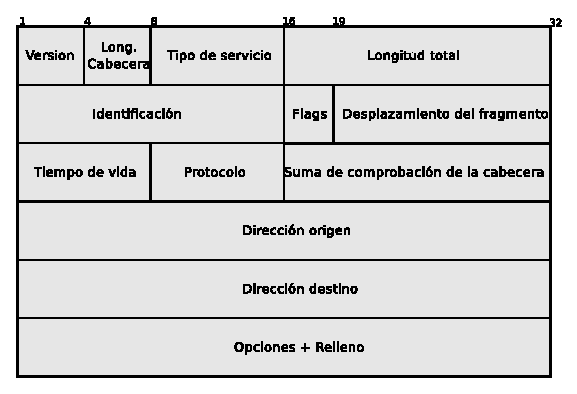
\includegraphics[width=1\textwidth]{2-sistema/graf/ip.eps}
  \caption{Formato de datagrama IP}
  \label{fig:ip}
\end{figure}

La PDU del protocolo IP se denomina \textit{datagrama IP} y se compone de los siguientes campos:
\begin{itemize}
	\item Versión: indica la versión del protocolo.
	\item Longitud de la cabecera: longitud de la cabecera expresada en palabras de 32 bits.
	\item Tipo de servicio: especifica los parámetros de fiabilidad, prioridad, retardo y rendimiento.
	\item Longitud total: longitud total del datagrama en Bytes.
	\item Identificador: un número de secuencia que, junto a la dirección origen y destino y el protocolo usuario, se utiliza para identificar de forma unívoca al datagrama.
	\item Flags: son 3 bits de los cuales solo 2 están definidos. El bit de \textit{no fragmentación} prohíbe la fragmentación cuando está puesto a 1. El bit de \textit{Más datos} se utiliza para fragmentación y reensamblado.
	\item Desplazamiento del fragmento: indica el lugar donde se sitúa el fragmento dentro del datagrama original, medido en unidades de 64 bits.
	\item Tiempo de vida: en cada router se decrementa en 1 unidad. Tiene como fin evitar que un datagrama se quede dando vueltas para siempre en la red.
	\item Protocolo: especifica a que protocolo del nivel de transporte corresponde el datagrama.
	\item Suma de comprobación de la cabecera: Es el complemento a uno de la suma en complemento a uno de todas las palabras de 16 bits de la cabecera.
	\item Dirección origen: codificada para permitir una asignación variable de bits para especificar la red y el sistema final conectado a la red especificada.
	\item Dirección destino: igual que el campo anterior.
	\item Opciones: contiene las opciones solicitadas por el usuario que envía los datos.
	\item Relleno: se usa para asegurar que la cabecera del datagrama tenga una longitud múltiplo de 31 bits.
	\item Datos: debe tener una longitud múltiplo de 8 bits.
\end{itemize}

\subsubsection{Dirección IP}

Es un número de 32 bit que identifica un dispositivo dentro de una red que utilice el protocolo IP. Las direcciones IP se suelen representar por cuatro números decimales separados por puntos, que equivalen al valor de cada uno de los cuatro bytes que componen la dirección.

Como ocurre en la mayoría de las redes las direcciones IP tienen una estructura jerárquica. Una parte de la dirección corresponde a la red, y la otra al host dentro de la red. Cuando un dispositivo de enrutamiento recibe un datagrama por una de sus interfaces compara la parte de red de la dirección con las entradas contenidas en sus tablas (que normalmente sólo contienen direcciones de red, no de host) y envía el datagrama por la interfaz correspondiente.

Los bits que corresponden a la parte de red conforman lo que se denomina \textit{prefijo de red}.

Existen 3 maneras de representar un prefijo de red:

\begin{itemize}
	\item Binario con asterisco: por ejemplo, el prefijo 132.239 se denotaría 1000010011101111* (dado que 132 es en binario 10000100 y 239 es 11101111). El asterisco al final denota que los bits restantes pueden ser de cualquier valor.
	\item Notación A/L, donde A es una dirección IP y L es la longitud del prefijo. Siguiendo el ejemplo anterior, la notación sería 132.239.0.0/16.
	\item Notación máscara: pe utiliza una dirección de red y una máscara en vez de un prefijo explícito. De esta manera, volviendo al ejemplo anteriormente mencionado, éste puede expresarse como 132.239.0.0 con máscara 255.255.0.0
\end{itemize}
\end{comment}

La necesidad de procesar cada vez más paquetes de datos lleva a lo que se conoce como clasificación.

\subsubsection{Clasificación}
El proceso de categorización de paquetes en flujos se denomina \textbf{clasificación}. Ésta se efectúa en base a un número de campos en la cabecera del paquete, tales como la dirección de origen/destino, puerto de origen/destino, tipo de servicio (TOS), etc. En general, para una clasificación basada en N campos, se dice que la misma es N-dimensional (o multidimensional). El propósito de la misma es clasificar paquetes de acuerdo a un conjunto de reglas dado.

Cada regla \textbf{R} tiene \textbf{F} componentes y el $ f^{vo} $ componente de \textbf{R}, denotado como \textbf{R[f]} es una \textit{expresión de correspondencia de rango} en el $ f^{vo} $ campo del paquete. Si para todo \textit{f} $ \in $ [1, \textit{f}] el $ f^{vo} $ campo de la cabecera de un paquete \textbf{P} satisface la expresión de rango \textbf{R[f]}, \textbf{P} se corresponde con \textbf{R}.

Un caso particular de clasificación unidimensional es lo que se conoce como Lookup. 

\subsubsection{Lookup}

El procedimiento que se lleva acabo en un dispositivo de enrutamiento podría describirse de la siguiente manera:

Un paquete llega por una interfaz de entrada. Éste porta una dirección IP determinada. El dispositivo consulta una tabla de forwardeo para determinar la interfaz de salida para el paquete en cuestión. Dicha tabla contiene un conjunto de prefijos con sus correspondientes interfaces de salida. El paquete es correspondido con el prefijo más largo que esté contenido en la dirección de destino y luego es redirigido  a la correspondiente interfaz de salida. Esta tarea de determinar el enlace de salida es denominada \textit{Búsqueda de dirección (address lookup).}




\section{Objetivos}
\subsection{Objetivos Generales}
Teniendo en cuenta los problemas planteados, el objetivo general de este proyecto es estudiar los diversos algoritmos de clasificacion de paquetes para poder encontrar las limitaciones en la implementacion de los mismos tanto en software como en hardware. 
En Particular, se pretende considerar una plataforma de logica reconfigurable que permite intergar arquitecturas de Hardware con Software embebido.

\subsection{Objetivos Especificos}
\begin{itemize}
	\item Implementar un sistema embebido que realice la clasificiación unidimensional de paquetes mediante una arquitectura mixta, Hardware-Software, en lógica reprogramable y que permita contratastar algunos de los algoritmos de clasificacion existentes. Dicho sistema debe recibir paquetes ethernet y procesarlos mediante información de control de tal forma que entregue a la salida paquetes factibles de ser colocados en diferentes flujos.
	\item Implementar como mínimo dos algoritmos de clasificación. Se deberá evitar el uso de recursividad, procurando alcanzar el mejor timing posible para cada paquete entrante.
	\item Mejorar las algoritmos anteriormente mencionados, poniendo el foco en optimizar el código.
\end{itemize}

\section{Organizacion}
+Estructura del Informe y breve descripcion de los capitulos





%\section{Distribucion Lineal}
